% Chapter Template

\chapter{Methods}\label{Methods} % for referencing this chapter elsewhere, use \ref{Methods}

%----------------------------------------------------------------------------------------
%	SECTION 1
%----------------------------------------------------------------------------------------

\section{NMF}

Non-Negative Matrix Factorization is the statistical framework in which this analysis is based on. Given a non-negative matrix \(V\), NMF is an unsupervised learning method which tries to find non-negative matrix factors \(W\) and \(H\) such that

\begin{equation}
     V \approx W \times H.
\end{equation}

The epigenetic data used, described in a later section \ref{data}, fulfills the precondition of non-negativity of the data. The \(V\) matrix used in the analysis is composed by 200-bp bins as rows and the epigenetic marks as columns. We are investigating the possibility of finding \(k\) signatures which will summarize combinatorial patterns of the data to the epigenetic marks by means of the \(H\) matrix and to the genome-wide bins by means of the \(W\) matrix.

\medskip

In order to perform the analysis, the \(V\) matrix was loaded into R environment and concretely the Rpackage \textit{NMF} was used \cite{Gaujoux2010}. The package used was select for consistency with previous similar studies \cite{Gandolfi2017} and seeing that attempts to implement the algorithm resulted in more time-consuming alternatives. Rpackage \textit{NMF} offers a framework with several NMF algorithms, including the ones explained in a previous section \ref{NMFalgs}, from which \texttt{brunet} option was chosen. This algorithm is based on Kullback-Leibler divergence and matches the one described in \cite{Lee2001} and used in \cite{Brunet2004}, enhanced to avoid numerical overflow.

%-----------------------------------
%	SUBSECTION 1
%-----------------------------------
\subsection{Algorithm}

Passed on a non-negative matrix \(V\) of \(m \times n\) size and a chosen number of \(k\) signatures, \texttt{brunet} implementation will find the approximation \(V \approx WH\).

\begin{enumerate}
    \item First, both \(W\) and \(H\) matrices are randomly initialized.
    \item Then, every row in \(W\) is updated according to the correspondent multiplicative update rules mentioned in (1.7).
    \item Every column in \(H\) is updated according to (1.6).
    \item Repeat steps 2 and 3 until the default convergence criteria is reached.
\end{enumerate}

The stopping or convergence criteria for the NMF algorithm can be based on a fixed number of iterations or the invariability of the target values \[( \vert \vert WH \vert \vert  )_t = ( \vert \vert WH \vert \vert  )_{t+1}.\] Since no fixed number of iterations was assumed, the stopping criteria for the analysis was the invariability of the \(WH\) matrix multiplication, which means there were different number of iterations when NMF was applied to the alternative tissues, varying between 350-600 iterations. The implementation in \textit{NMF} package includes parallel computations to speed up the process.

%-----------------------------------
%	SUBSECTION 2
%-----------------------------------

\subsection{Choosing number of signatures}\label{chooseK}

In order to apply NMF to the data we foremost need to choose a suitable \(k\) number of signatures, also called rank. The number of clusters defined will largely influence the results and the explanation of them, therefore it is highly important to find the optimal number to produce ``meaningful'' clusters \cite{Brunet2004}. As explained in previous sections, there is no standard procedure to find the best \(k\) number. Therefore, an additional matrix was created with randomly permuted values from the original \(V\) matrix, which we will refer to as ``random'' \(V_R\) matrix. The \(V_R\) matrix is composed of the same values as \(V\) but column-wise permuted, meaning that the presumed chromatic patterns would not be able to be recognized.

\begin{figure}[h]
    \centering
    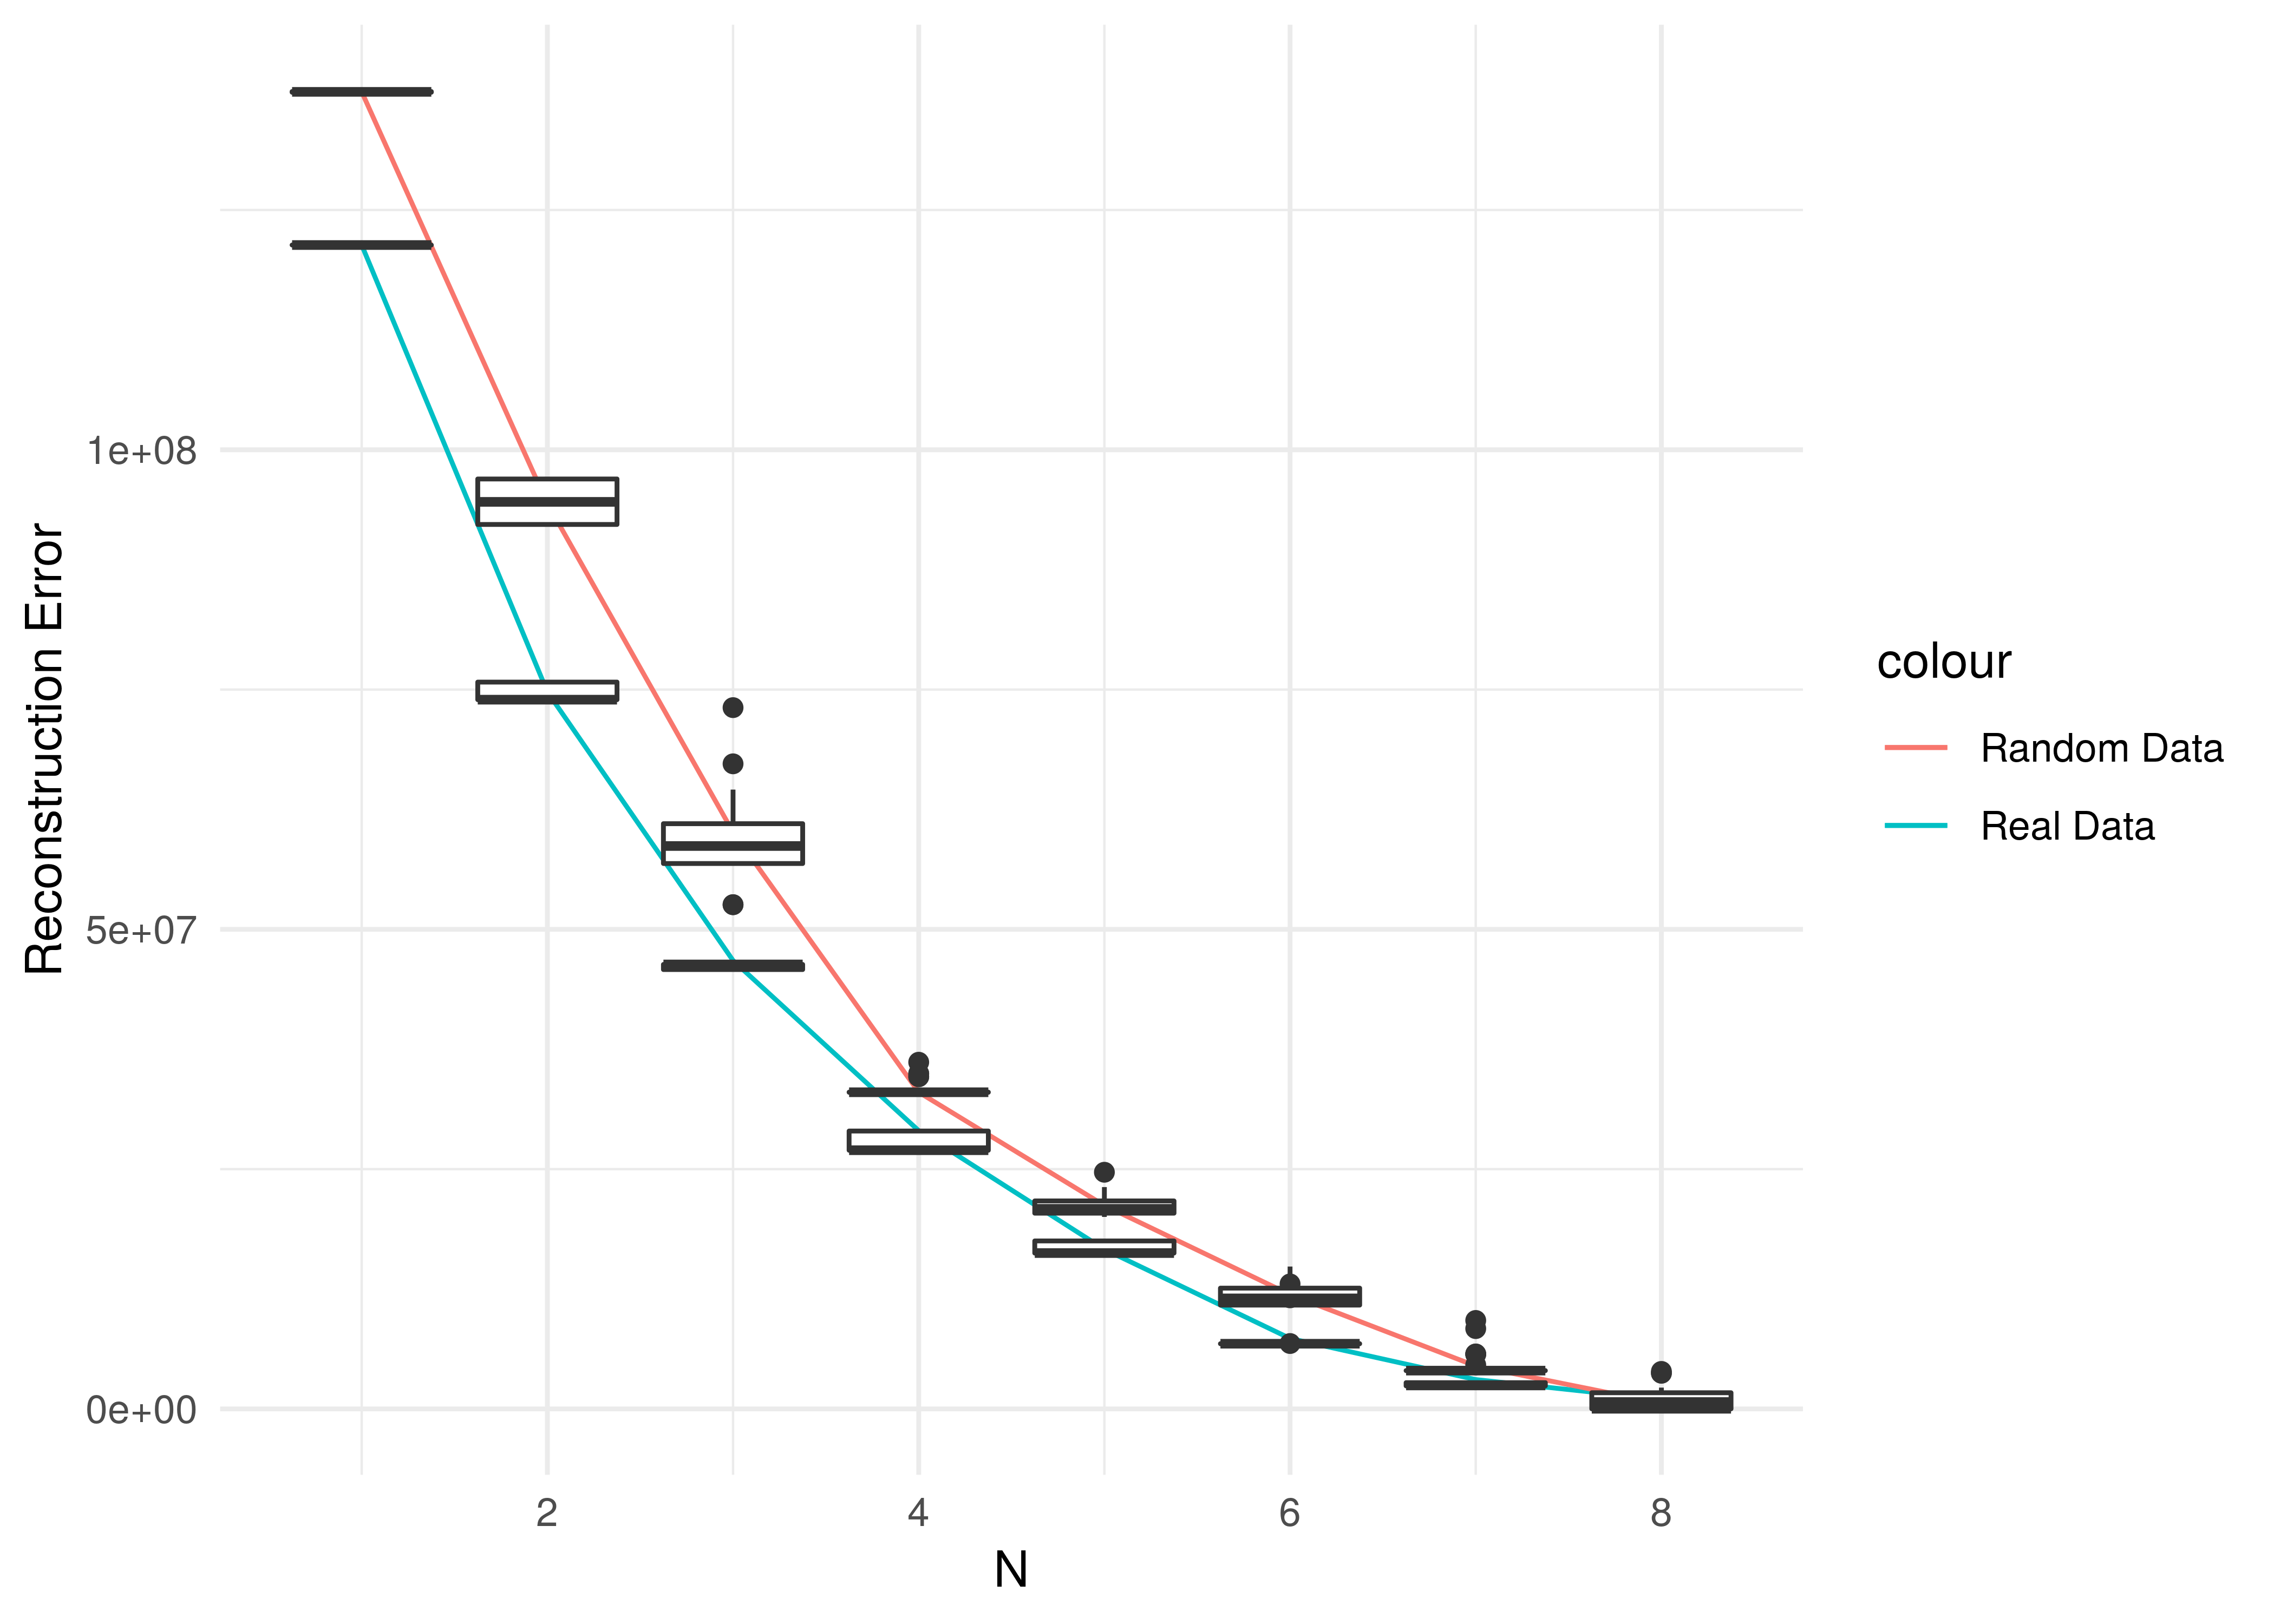
\includegraphics[width=0.7\linewidth]{Figures/select_n/error_by_n.png}
    \caption[Reconstruction error by k value]{\textbf{Reconstruction error by k value}. The plot is used in order to choose the number of \(k\) signatures. For this purpose, the Residual Sum of Squares between the original values in \(V\) and the estimated values from \(W \times H\) were calculated for 30 iterations. The boxplots are constructed with every value from this 30 iterations and the lines represent the mean RSS value with every \(k\) value tested. Real data is represented in blue and random data is represented in red.}
    \label{fig:chooseK_error}
\end{figure}

\medskip

To compare the performance of NMF using different \(k\) values, the analysis is performed using values from 1 to 8 and then compared the reconstruction errors of the resultant models. As the NMF factorized matrix can vary from one run to another, the process is repeated 30 times and the results can be seen in Figure~\ref{fig:chooseK_error}. The reconstruction error was calculated for comparison by residuals sum of squares (RSS),

\begin{equation}
    \vert \vert V - WH \vert \vert ^ 2 = \sum_{ij} (V_{ij} - (WH)_{ij} )^2
\end{equation}

\medskip

As we can see from the results, for the same \(k\) value, the NMF model produces worst results for the \(V_R\) matrix as well as more variable results. Nevertheless, there is a \(k\) value for which the plots intersect due to the model being over-fitted. We chose \(k = 7\) because it is the value for which the reconstruction error is the lowest possible before modeling the noise in the data. The results found similar in all the three cell types.

%----------------------------------------------------------------------------------------
%	SECTION 3
%----------------------------------------------------------------------------------------

\section{Data}\label{data}

The data used in this study was obtained entirely from the ENCODE project database \cite{Feingold2004}, where multiple epigenetic marks and reference epigenomes are available. Data sets from 11 types of epigenetic marks were collected, including histone modifications (H3K4me3, H3K4me1, H3K27ac, H3K36me3, H3K9me3, H3K27me3 and H3K9ac), chromatin remodeling proteins (EP300 and H2A.Z) and transcription regulation factors (CTCF, POLR2A). Replicate samples for each of the 11 epigenetic marks were used in the three cell lines of study, which includes a human liver cancer cell line (HepG2) \cite{Aden1979}, myelogenous leukemia cell line (K562) \cite{Andersson1979} and cells derived from HeLa cancerous cervical tumor line (HeLa-S3) \cite{Douglas1973,Chen2008}.

\medskip

In order to standardize the input and facilitate the data sets processing, the information for all the samples was arranged in a tab separated file with the following fields as columns:

\begin{enumerate}
    \item \textbf{Cell line type}. Either HepG2, K562 or Hela-S3 for this analysis.
    \item \textbf{Epigenetic modification category}. Where does the modification apply. Either histone modification (`histonemod'), chromatin modulation (`openchromatin') or transcription factor (`TFBS').
    \item \textbf{Epigenetic modification name}. The label of the mark which the sample corresponds to, as mentioned above.
    \item \textbf{Accession ID}. The accession name for the sample in the database.
    \item \textbf{File name}.
    \item \textbf{Processing status}. Either `raw' or `process'. Raw samples need to be pre-processed.
    \item \textbf{Replicate number}. Integer enumerating the various replicates for a particular epigenetic mark.
    \item \textbf{Database name}. In the present case, `ENCODE'.
    \item \textbf{Download link}. Used to download the sample reads file.
\end{enumerate}

As a matter of convenience, `\path{downloadData.sh} \path{[DataInfo.tsv]}' or `\path{epigeNMF.sh} \path{-d}  \path{[DataInfo.tsv]}' can be used to automatically download the data sets into the appropriate directory tree: \path{CELL_LINE/SIGNAL_TRACK/SAMPLE_ID}.

%----------------------------------------------------------------------------------------
%	SECTION 3
%----------------------------------------------------------------------------------------

\section{Pipeline}

In order to integrate the different scripts used in the project, a bash command line tool was created. The command line requires of a conda environment which can be set up using the \texttt{createCondaEnv.sh} script. This command line includes options to follow the next pipeline for the analysis:

\begin{enumerate}
    \item Download the data (option \texttt{-d} or \texttt{--download}).
    \item Prepare BED alignment files (option \texttt{-p} or \texttt{--process}).
    \item Create V matrix of counts for marks (cols) by bins (rows) (option \texttt{-c} or \texttt{--counts}).
    \item Filter V matrix bins to remove noise (option \texttt{-f} or \texttt{--filter}).
    \item Choose the optimal `n' number of signatures for NMF (option \texttt{-k} or \texttt{--chooseN}).
    \item NMF analysis (option \texttt{-n} or \texttt{--nmf}).
\end{enumerate}

All the scripts used for the analysis as well as for creating the report are available as a \href{https://bitbucket.org/alekssro/mscthesis/src/master/}{Bitbucket repository}.

\subsection{Download Data}

Command: \texttt{scripts/epigeNMF.sh -d [Datasets.tsv]}

\smallskip

Makes use of \texttt{downloadData.sh} script. It requires the file with the datasets info as explained in the Data section \ref{data}. For each sample, the dataset will be downloaded and saved in the \path{data} directory using the next file tree: \path{data/[cell_line]/[epigenetic_mark_name]/[sample_id]/}.

\subsection{Processing BAM files}

Command: \texttt{scripts/epigeNMF.sh -p [Datasets.tsv]}

\smallskip

Makes use of \texttt{prepareBedAlignment.sh} script, based on the processing pipeline used in \cite{Gandolfi2017}, following the scheme and updating outdated methods. The script process raw BAM files into filtered BED files by (1) removing duplicate reads, (2) filter reads by quality, (3) add a 200-bp tag extension in both 3' ends to transcription factors and histone modification signals (resembling half of the average ChIP-seq fragments) and (4) convert BAM files into BED files. It outputs processed BED files to the same path as the BAM file.

\subsection{Generate V matrix}

Command: \texttt{scripts/epigeNMF.sh -c [cell-lines]}

\smallskip

Calls \texttt{bedToNormCounts.sh} script, based on the processing pipeline used in \cite{Gandolfi2017}, following the scheme and updating outdated methods. Takes the cell lines desired to generate the \(V\) matrix from their samples. It requires the datasets info file, human genome segmented into 200-bp fragments as well as a uniqueness mappability track file (using the reference \textit{Duke Uniqueness Regions}) to be in the data directory. For each sample in each cell line, the script assigns the reads to a bin in the segmented genome and calls \texttt{bedCountsToV.R} script which adds the columns of the corresponding cell line \(V\) matrix.

\medskip

The bin counts are normalized with an scaling factor based on the uniqueness mappability positions present in each bin and the total number of reads in the sample. The technical replicates available for a epigenetic sample were combined by taking the mean of the normalized counts for each bin. The result of the execution is a \(V\) matrix csv file for each of the cell lines of interest, saved in the file tree directory \path{results/genomic_survey/[cell_line]/V_matrix.csv}.

\subsection{Filter V matrix}

Command: \texttt{scripts/epigeNMF.sh -f [input-V.csv] [output-V.csv]}

\smallskip

Uses \texttt{summariseFilterData.R} script. Takes as arguments the input and output directories, being the input an unfiltered \(V\) matrix in CSV format and the output a \(V\) filtered matrix also in CSV format. The bins are filtered taking only those for which at least one of the epigenetic marks fall into the top 2.5\% percentile. The threshold was set to the 0.975 quantile in order to filter out the counts considered as noise for our analysis.

\subsection{Choose number of signatures}

Command: \texttt{scripts/epigeNMF.sh -k [input] [output] [n-repeats]}

\smallskip

With \texttt{chooseN.R} script used to choose the optimal \(k\) number of signatures for the NMF analysis in the filtered \(V\) matrix data. Generates a plot comparing real and random data reconstruction errors (choose \(k\) based on that). It also includes an option to define the number of times NMF and reconstruction error are calculated for each \(k\) value. Outputs a residual error plot as the one described in \ref{chooseK} section.

\subsection{NMF analysis}

Command: \texttt{scripts/epigeNMF.sh -n [input-file] [output-file] [n-signatures]}

\smallskip

Calls \texttt{NMFanalysis.R} with a filtered \(V\) matrix in CSV file as input, and produces several informative plots describing the \(H\) and \(W\) matrices generated, saving them to the output directory. The number of signatures can be passed as an argument, with a default of \(k = 7\).

%----------------------------------------------------------------------------------------
%	SECTION 4
%----------------------------------------------------------------------------------------

\section{Performance}

During the project, around 150 GB of sequencing data were downloaded, processed and analyzed. Therefore, it was crucial to use the high-performance computing facility provided by GenomeDK at Aarhus University. In particular, nodes with 64 GB of RAM were used. The large amount of data used made the task computationally intensive and some performance test were done.

\medskip

Pre-processing the data takes the major part of the time which could be avoided by saving the processed files into a database. It would also be possible to optimize the algorithm in the process of assigning the read counts for each bin. In any case, the whole process took approximately 8-10 hours of computation for the 87 ChIP-seq alignments used, using the mentioned computational cluster. Once the \(V\) matrices are generated, the NMF method lasted no more than 5 minutes to run.

\subsection{Pre-processing}

As mentioned, this is the most time-consuming step of the process. Figure~\ref{fig:PreProcess} shows the time it took for each read in the input to process the data. With changing numbers of reads (\textit{N}), the pre-processing time exhibits an asymptotic flat curve when the input size is in logarithmic. The time in seconds is divided by the input size (number of ChIP-seq reads), in order to get the time for each read. Consequently, the algorithm seems to perform in an \(\mathcal{O}(n \log{n})\) fashion, which can be caused by the indexing and sorting carried out in this step.

\begin{figure}[h]
    \centering
    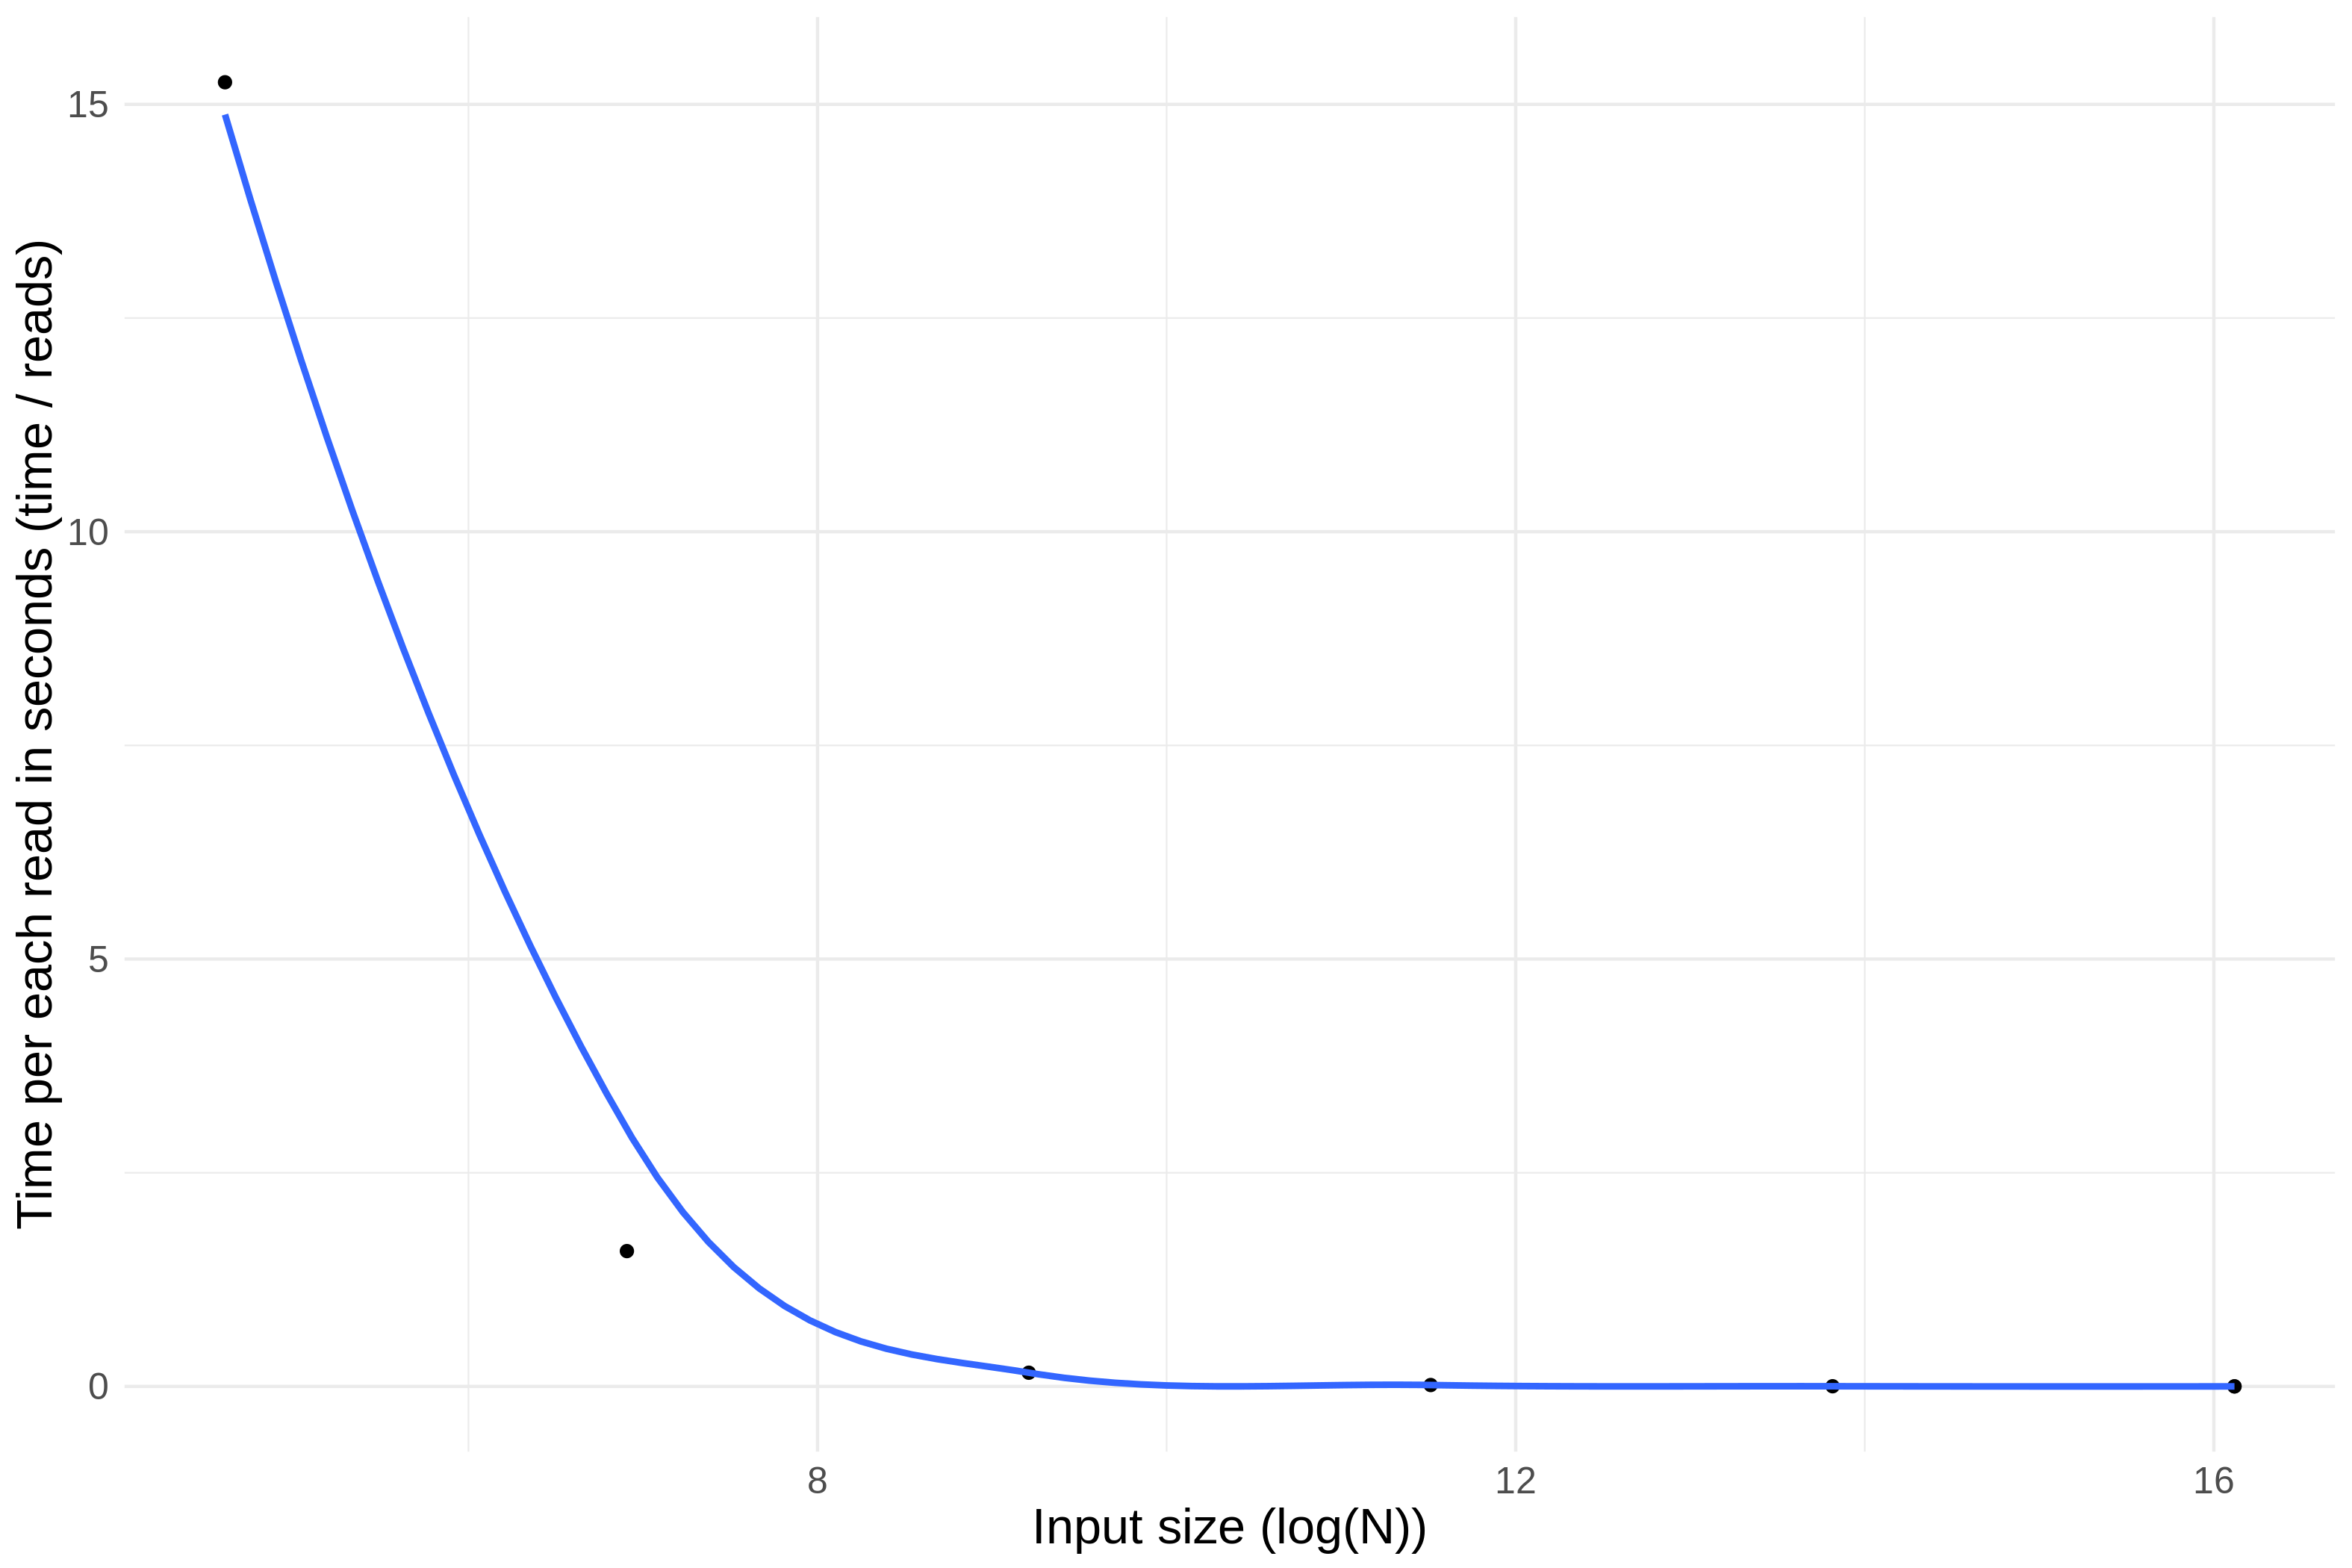
\includegraphics[height=8cm]{Figures/performance/performance_per_read.png}
    \caption[Pre-processing performance by read]{\textbf{Pre-processing performance by read}. Multiple input sizes were used in order to time the execution of the pre-processing script. The figure summarise the results from those multiple runs. The x axis is in logarithmic scale, being the input size as \(\log(N)\). The data points shown are the result from dividing the time in seconds by the number of reads.}
    \label{fig:PreProcess}
\end{figure}

\medskip

\subsection{NMF analysis}

The NMF analysis is the cornerstone of the presented master thesis. Considering the high-dimensionality of the data, it is important that the method is able to find the signatures on the data with an acceptable performance. Additionally, we need to choose the \(k\) signatures used, and the way this number is chosen requires to perform NMF for every \(k\) value tested. Consequently, here we performed tests both to investigate the performance of the NMF with changing number of signatures \(k\), and with different number of bins input. Figure~\ref{fig:NMF}A shows how the different k values affect the running time and Figure~\ref{fig:NMF}B represents the performance dependent on the input size.

\begin{figure}[h]
    \centering
    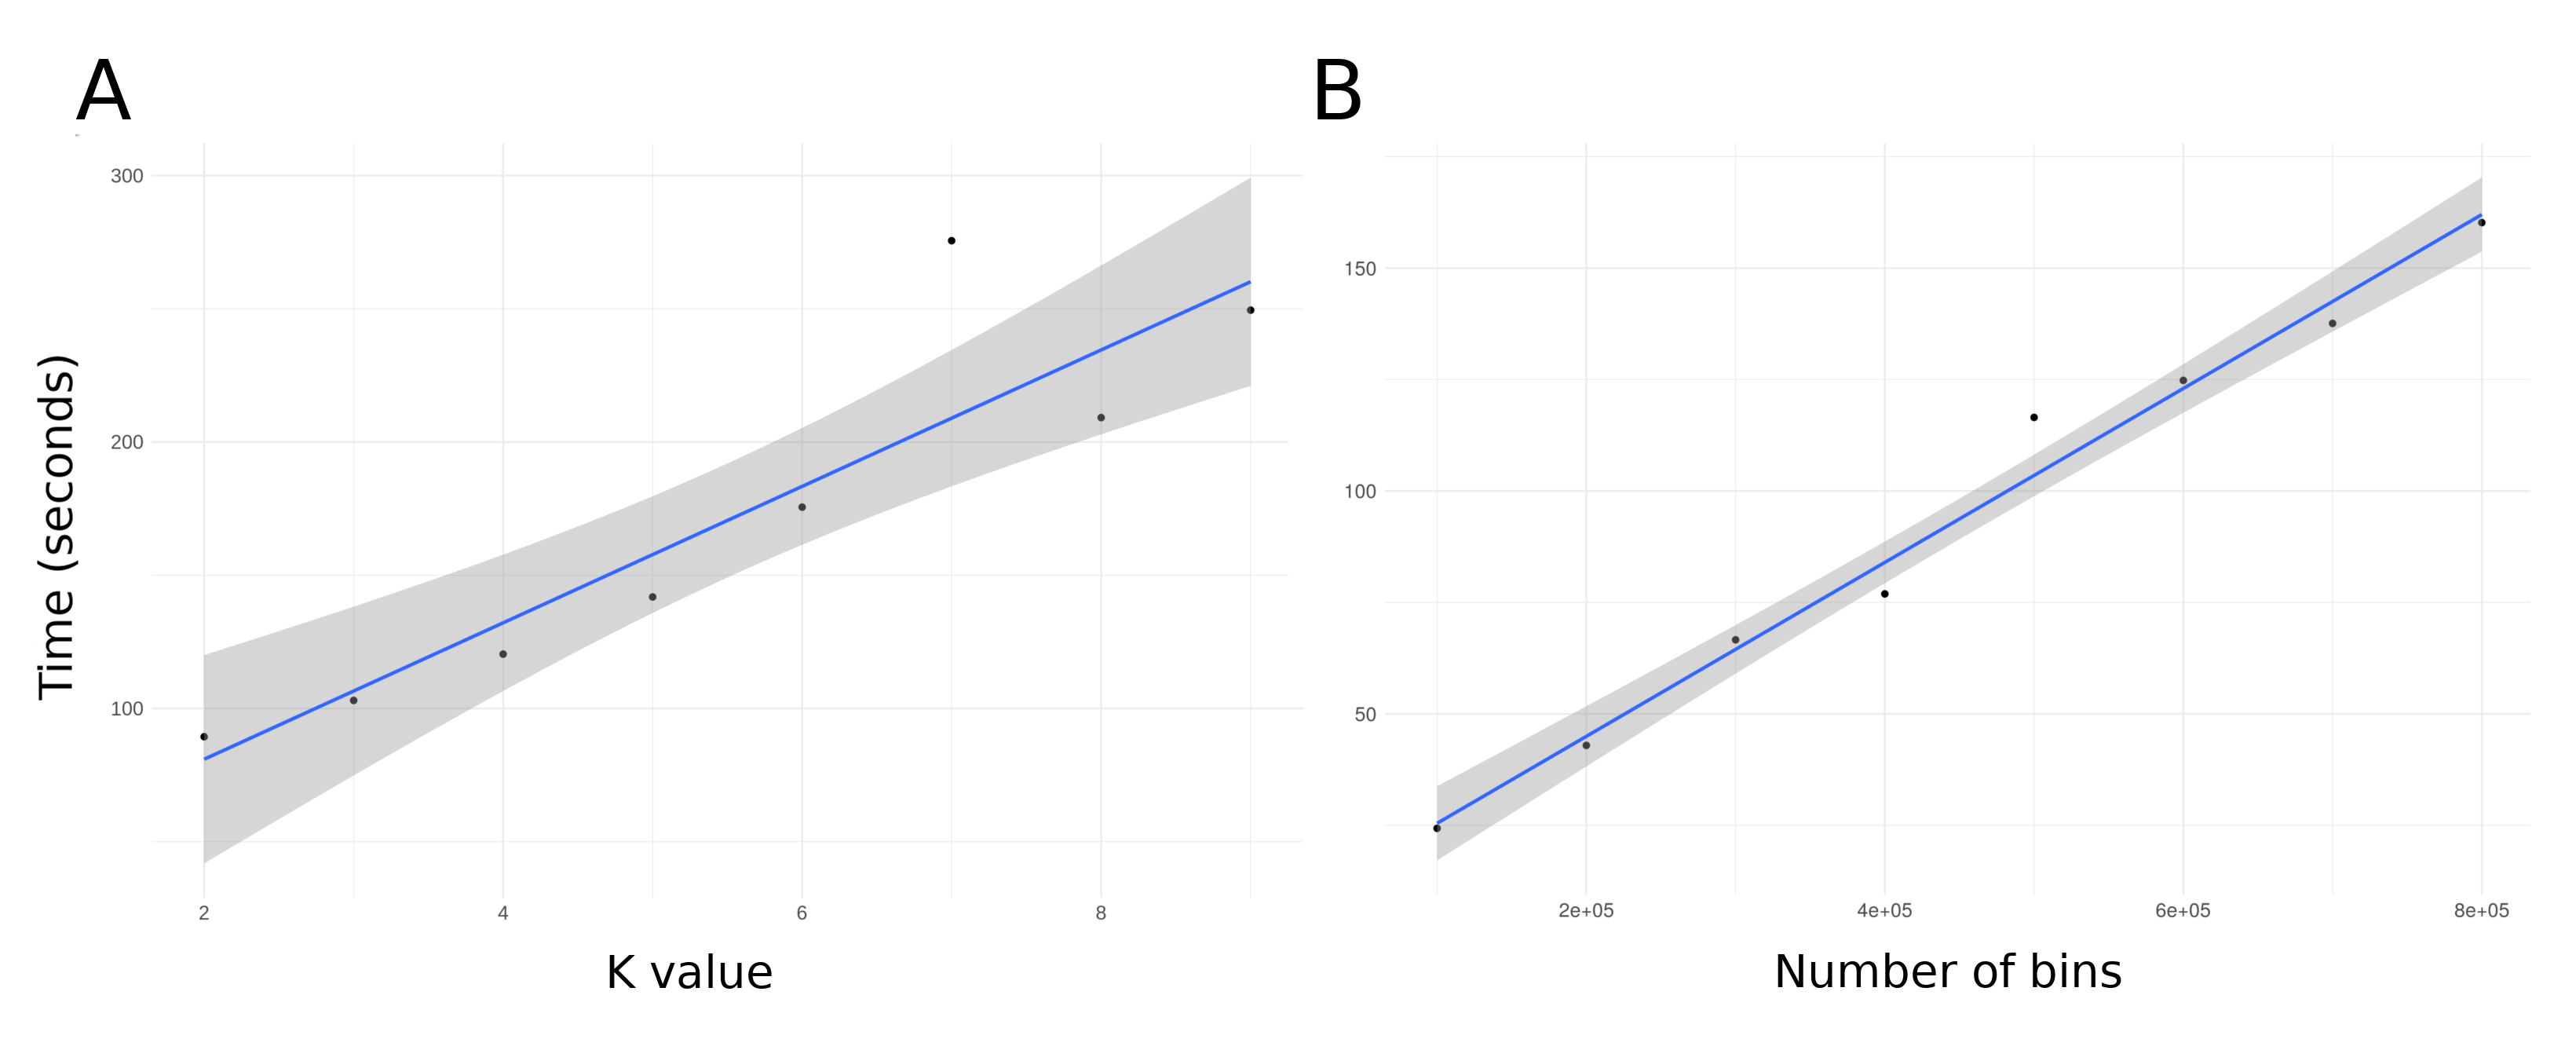
\includegraphics[width=\textwidth]{Figures/performance/performance_nmf_join.png}
    \caption[NMF performance]{\textbf{NMF performance}. Studying the performance of the NMF, we have to take into account two possible factors: \textbf{A}: Performance as time in seconds of the NMF algorithm for different number of signatures (\(k\)). \textbf{B}: Performance as time in seconds of the NMF algorithm for changing number of bins (\(N\))}
    \label{fig:NMF}
\end{figure}

\medskip

Both plots suggest a linear time complexity behavior \(\mathcal{O}(n)\). It is important to take into account the stopping criteria used for the NMF, as it is based in convergence. The convergence of the algorithm can vary slightly from one run to another and it is revealed as some points lay out of the standard error boundary. However, the running times show that even with the full data \((\sim800,000)\) and using a personal computer the task run in short time.
